\section{実験概要}
本研究で作成したドキュメントの有効性を確認するため, つくばチャレンジ2025\cite{つくばチャレンジ}のコースを用いて自律移動実験を行った. 
実験では, ドキュメントによる手順通りにナビゲーションのパラメータを調整されたロボットが, 自律的に設定されたコースを完走できるかで, ドキュメントの有用性を確認することを目的とした. 
そのコースを\figref{Fig:Course map of the Tsukuba Challenge 2025}に示す.
実験では, 作成者が走行地図の作成から自己位置推定および経路計画に関する各種パラメータの調整までを全て行った. 
また, LiDARの計測値が一定の閾値以下になったときに減速, 停止を行う処理や, 
特定の場所で一時的にコストマップを無効化する処理, ロボットがスタックしたときにコストマップを初期化する処理といった補助的なノードを併用した. これらは, 
人やロボットなどの動的障害物が多いつくばチャレンジにおける自律移動上の拡張として導入した. 

実験には, 本研究室で開発されているロボットORNE-box2を使用した. 
また, ナビゲーションにはROS Navigation stackを用いた. 
\begin{figure}[hbtp]
  \centering
 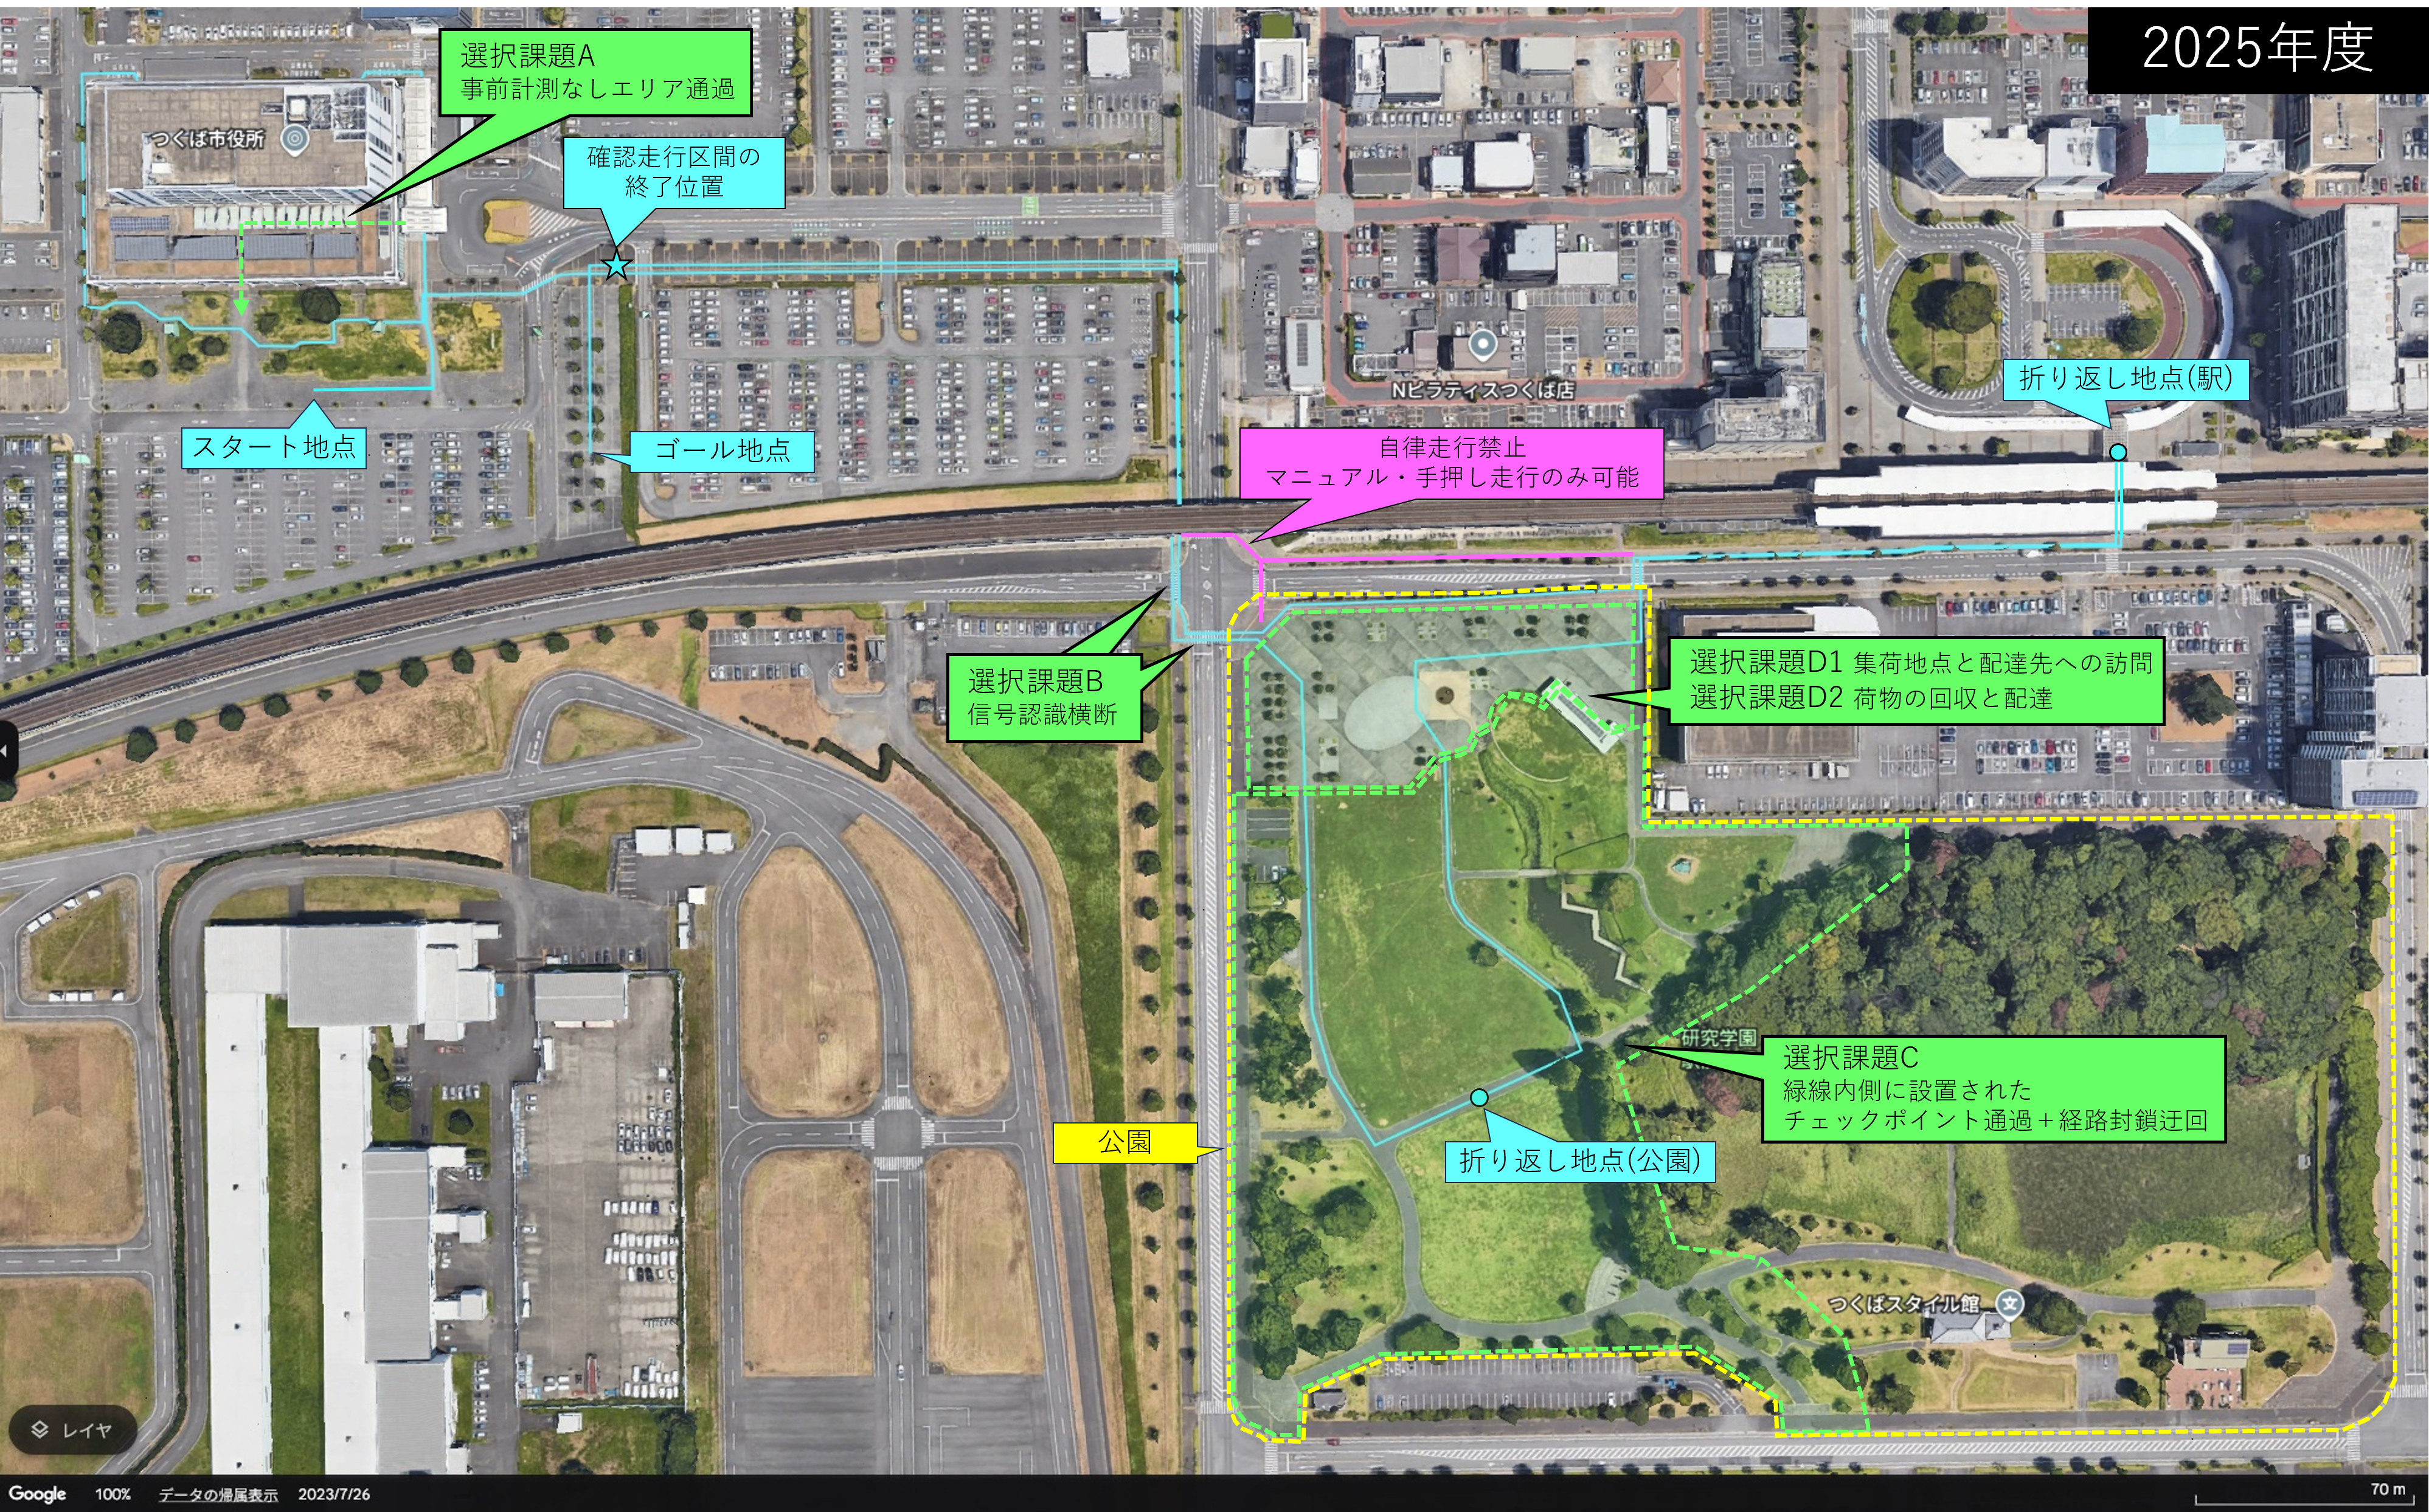
\includegraphics[keepaspectratio, scale=0.3]
      {images/course_2025.png}
 \caption{Course map of the Tsukuba Challenge 2025(souce: \cite{つくばチャレンジ})}
 \label{Fig:Course map of the Tsukuba Challenge 2025}
\end{figure}

\newpage
\section{実験結果}
% 表
\tabref{}に示すように, 